\documentclass{article}

% if you need to pass options to natbib, use, e.g.:
% \PassOptionsToPackage{numbers, compress}{natbib}
% before loading nips_2018

% ready for submission
\usepackage{nips_2018}

% to compile a preprint version, e.g., for submission to arXiv, add
% add the [preprint] option:
% \usepackage[preprint]{nips_2018}

% to compile a camera-ready version, add the [final] option, e.g.:
% \usepackage[final]{nips_2018}

% to avoid loading the natbib package, add option nonatbib:
% \usepackage[nonatbib]{nips_2018}

\usepackage[utf8]{inputenc} % allow utf-8 input
\usepackage[T1]{fontenc}    % use 8-bit T1 fonts
\usepackage{hyperref}       % hyperlinks
\usepackage{url}            % simple URL typesetting
\usepackage{booktabs}       % professional-quality tables
\usepackage{amsfonts}       % blackboard math symbols
\usepackage{nicefrac}       % compact symbols for 1/2, etc.
\usepackage{microtype}      % microtypography
\usepackage{amsmath}
\usepackage{amssymb}
\usepackage{amsthm}
\usepackage{bm}
\usepackage{todonotes}
\usepackage{algorithm}
\usepackage{algorithmic}
\usepackage{thmtools, thm-restate}

\newtheorem{lemma}{Lemma}
\newtheorem{theorem}{Theorem}
\newtheorem{corollary}{Corollary}
\newtheorem{remark}{Remark}
\newtheorem{definition}{Definition}
\newtheorem{proposition}{Proposition}

\newcommand{\argmin}{\operatornamewithlimits{argmin}}
\newcommand{\argmax}{\operatornamewithlimits{argmax}}
\newcommand{\mm}{\operatornamewithlimits{mm}}
\newcommand{\wt}[1]{\widetilde{#1}}
\newcommand{\wh}[1]{\widehat{#1}}
\newcommand{\norm}[1]{\left\lVert #1 \right\rVert}
\newcommand{\abs}[1]{\left\lvert #1 \right\rvert}
\title{What the hell is the title of this paper?}

% The \author macro works with any number of authors. There are two
% commands used to separate the names and addresses of multiple
% authors: \And and \AND.
%
% Using \And between authors leaves it to LaTeX to determine where to
% break the lines. Using \AND forces a line break at that point. So,
% if LaTeX puts 3 of 4 authors names on the first line, and the last
% on the second line, try using \AND instead of \And before the third
% author name.

\author{
  David S.~Hippocampus\thanks{Use footnote for providing further
    information about author (webpage, alternative
    address)---\emph{not} for acknowledging funding agencies.} \\
  Department of Computer Science\\
  Cranberry-Lemon University\\
  Pittsburgh, PA 15213 \\
  \texttt{hippo@cs.cranberry-lemon.edu} \\
  %% examples of more authors
  %% \And
  %% Coauthor \\
  %% Affiliation \\
  %% Address \\
  %% \texttt{email} \\
  %% \AND
  %% Coauthor \\
  %% Affiliation \\
  %% Address \\
  %% \texttt{email} \\
  %% \And
  %% Coauthor \\
  %% Affiliation \\
  %% Address \\
  %% \texttt{email} \\
  %% \And
  %% Coauthor \\
  %% Affiliation \\
  %% Address \\
  %% \texttt{email} \\
}

\begin{document}
% \nipsfinalcopy is no longer used

\maketitle

\begin{abstract}
  The abstract paragraph should be indented \nicefrac{1}{2}~inch
  (3~picas) on both the left- and right-hand margins. Use 10~point
  type, with a vertical spacing (leading) of 11~points.  The word
  \textbf{Abstract} must be centered, bold, and in point size 12. Two
  line spaces precede the abstract. The abstract must be limited to
  one paragraph.
\end{abstract}

\section{Introduction}

Recent advances have allowed reinforcement learning (RL) \cite{} to achieve impressive results in a wide variety of complex tasks, ranging from Atari \cite{}, to the game of Go \cite{}, to the control of sophisticated robotics systems \cite{}. The main limitation is that RL algorithms still require an enormous amount of experience samples before successfully learning such complicated tasks. One of the most promising solutions is transfer learning, which focuses on reusing past knowledge available to the agent in order to reduce the sample-complexity for learning new tasks. In the typical settings of transfer in RL \cite{}, the agent is assumed to have already solved a set of \textit{source tasks} generated from some unknown distribution. Then, given a \textit{target task} drawn from the same distribution, or a slightly different one, the agent can rely on knowledge from the source tasks to speed-up the learning process. This constitutes a significant advantage over plain RL, where the agent learns each new task from scratch independently of previous learning experience. Several algorithms have been proposed in the literature to transfer experience samples \cite{}, policies/options \cite{}, rewards \cite{}, value functions \cite{}, features \cite{}, and so on. We refer the reader to \cite{} for a thorough survey on transfer in RL.

\paragraph*{Exploration-based introduction}
One of the most relevant problems in this context is how to efficiently explore the target task based on knowledge from the source tasks. Intuitively, assuming the tasks under consideration share some similarities due to the common distribution, much better exploration strategies than uninformed ones (e.g., $\epsilon$-greedy) can be adopted for quickly learning the target task. Among the appealing approaches for this problem we find Bayesian methods (e.g., \cite{}), which are able to model the uncertainty over the current task based on previous knowledge and drive exploration so that this uncertainty is reduced as quickly as possible. Similarly, model-based algorithms (e.g., \cite{}) typically transfer samples to improve their estimates of the task model and adopt classic count-based exploration to drive the agent towards regions where such estimates are more uncertain. However, all these approaches either require strong assumptions (for example, on the distribution involved in Bayesian methods) or do not scale well to large problems. This greatly limits their practical applicability.

In this work, we tackle such limitations by considering a more general approach. Similarly to \cite{}, we assume tasks to share similarities in their value functions and use the given source tasks to learn the distribution over such functions. Then, we use this distribution as a prior for learning the target task and we propose and efficient variational approximation of the corresponding posterior. Leveraging on recent ideas from randomized value functions (\cite{}), we design a Thompson sampling-based algorithm which efficiently explores the target task by repeatedly sampling from the posterior and acting greedily w.r.t. (with respect to) the sampled value function. We show that our approach is very general, in the sense that it does not require any specific choice of function approximator or prior/posterior distribution models. \todo[inline]{Maybe mention something about theory/experiments here}

\paragraph*{Transfer-based introduction}

Under the assumption that tasks follow a certain distribution, an intuitive choice for designing a transfer algorithm is to attempt at charactering the uncertainty over the target task. Then, an ideal algorithm would leverage prior knowledge from the source tasks to interact with the target task in such a way that this uncertainty is reduced as quickly as possible. This simple intuition makes Bayesian \todo{probabilistic? distributional?} methods appealing approaches for transfer in RL, and many previous works have been proposed in this direction. \cite{} assume tasks share similarities in their dynamics and rewards and propose a hierarchical Bayesian model for the distribution of this two elements. Similarly, \cite{} assume tasks are similar in their value functions and design a different hierarchical Bayesian model. More recently, \cite{}, and its extension \cite{}, consider tasks that share structure in their dynamics which is governed by some hidden parameters, and propose efficient Bayesian models for quickly learning such parameters in new tasks. However, all these algorithms require specific, and sometimes restrictive, assumptions (e.g., on the distributions involved or the function approximators adopted), which might limit their practical applicability. [Having more general algorithms that alleviate the need of strong assumptions and can be easily adapted to different contexts is one of the most relevant problems in current research.]

In this work, we take a more general approach. Similarly to \cite{}, we assume tasks to share similarities in their value functions and use the given source tasks to learn the distribution over such functions. Then, we use this distribution as a prior for learning the target task and we propose and efficient variational approximation of the corresponding posterior. Leveraging on recent ideas from randomized value functions (\cite{}), we design a Thompson sampling-based algorithm which efficiently explores the target task by repeatedly sampling from the posterior and acting greedily w.r.t. (with respect to) the sampled value function. We show that our approach is very general, in the sense that it does not require any specific choice of function approximator or prior/posterior distribution models. \todo[inline]{Maybe mention something about theory/experiments here}

The rest of this document is organized as follows... \todo[inline]{Complete this when the structure is defined or simply remove it to save space.}

\section{Preliminaries}

We define a Markov decision process (MDP) as a tuple $\mathcal{M} = \langle \mathcal{S},\mathcal{A},\mathcal{P},\mathcal{R},p_0,\gamma\rangle$, where $\mathcal{S}$ is the state-space, $\mathcal{A}$ is a finite set of actions, $\mathcal{P}(\cdot | s,a)$ is the distribution of the next state $s'$ given that action $a$ is taken in state $s$, $\mathcal{R}: \mathcal{S}\times\mathcal{A}\rightarrow\mathbb{R}$ is the reward function, $p_0$ is the initial-state distribution, and $\gamma\in [0,1)$ is the discount factor. We assume the reward function to be uniformly bounded by a constant $R_{max}>0$. A deterministic policy $\pi : \mathcal{S} \rightarrow \mathcal{A}$ is a mapping from states to actions. At the beginning of each episode of interaction, the initial state $s_0$ is drawn from $p_0$. Then, the agent takes the action $a_0 = \pi(s_0)$, receives a reward $\mathcal{R}(s_0,a_0)$, transitions to the next state $s_1 \sim \mathcal{P}(\cdot | s_0,a_0)$, and the process is repeated. The goal is to find the policy maximizing the long-term return over a possibly infinite horizon: $\max_{\pi}J(\pi)\triangleq\mathbb{E}[\sum_{t=0}^{\infty} \gamma^t r_t \mid \mathcal{M},\pi]$. To this end, we define the optimal value function $Q^*(s,a)$ as the expected return obtained by taking action $a$ in state $s$ and following an optimal policy thereafter. Then, an optimal policy $\pi^*$ is a policy that is greedy with respect to the optimal value function, i.e., $\pi^*(s) = \argmax_a Q^*(s,a)$ for all states $s$. It can be shown (e.g., \cite{puterman1994markov}) that $Q^*$ is the unique fixed-point of the optimal Bellman operator $T$ defined by $TQ(s,a) = \mathcal{R}(s,a) + \gamma\mathbb{E}_{\mathcal{P}}[\max_{a'}Q(s',a')]$ for any value function $Q$. From now on, we adopt the term $Q$-function to denote any plausible value function, i.e., any function $Q : \mathcal{S}\times\mathcal{A} \rightarrow \mathbb{R}$ uniformly bounded by $\frac{R_{max}}{1-\gamma}$.

When learning the optimal value function, a quantity of interest is how close a given $Q$-function is to the fixed-point of the Bellman operator. This is given by its Bellman residual, defined by $B(Q) \triangleq TQ - Q$. Notice that $Q$ is optimal if, and only if, $B(Q)(s,a) = 0$ for all $s,a$. Furthermore, if we assume the existence of a distribution $\nu$ over $\mathcal{S}\times\mathcal{A}$, the squared Bellman error of $Q$ is defined as the expected squared Bellman residual of $Q$ under $\nu$, $\norm{B(Q)}_{\nu}^2=\mathbb{E}_{\mu}\left[ B^2(Q) \right]$. Although minimizing the empirical Bellman error is an appealing objective, it is well-known that an unbiased estimator requires two independent samples of the next state $s'$ of each $s,a$ (e.g., \cite{} \todo{cite Maillard}). In practice, the empirical Bellman error is typically replaced by the TD error, which approximates the former using a single transition sample. Given a dataset of $N$ samples, the TD error is computed as $\norm{B(Q)}_{D}^2 = \frac{1}{N}\sum_{i=1}^N (r_i + \gamma \max_{a'} Q(s_i',a') - Q(s_i,a_i))^2$.

%\subsection{Variational Inference}
%
%When working with Bayesian approaches, the posterior distribution of hidden variables $\bm{w} \in \mathbb{R}^K$ given data $D$,
%\begin{equation}\label{eq:bayes}
%p(\bm{w} | D) = \frac{p(D | \bm{w})p(\bm{w})}{p(D)} = \frac{p(D | \bm{w})p(\bm{w})}{\int_{\bm{w}} p(D | \bm{w})p(\bm{w})},
%\end{equation}
%is typically intractable for many models of interest (e.g., when working with deep neural networks) due to difficulties in computing the integral of Eq. \eqref{eq:bayes}. The main intuition behind variational inference \cite{} \todo{CITE} is to approximate the intractable posterior $p(\bm{w} | D)$ with a simpler distribution $q_{\bm{\xi}}(\bm{w})$. The latter is chosen in a parametric family, with variational parameters $\bm{\xi}$, as the minimizer of the Kullback-Leibler (KL) divergence w.r.t. $p$:
%\begin{equation}
%\min_{\bm{\xi}} KL\left(q_{\bm{\xi}}(\bm{w})\ ||\ p(\bm{w} \mid D)\right)
%\end{equation}
%It is well-known that minimizing the KL divergence is equivalent to maximizing the so-called \textit{evidence lower bound} (ELBO), which is defined as:
%\begin{equation}
%\text{ELBO}(\bm{\xi}) = \mathbb{E}_{\bm{w} \sim q_{\bm{\xi}}}\left[ \log p(D | \bm{w}) \right] - KL\left(q_{\bm{\xi}}(\bm{w})\ ||\ p(\bm{w})\right)
%\end{equation}
%Intuitively, the best approximation is the one that maximizes the expected log-likelihood of the data, while minimizing the KL divergenge w.r.t. the prior $p(\bm{w})$.

\section{Variational Transfer Learning}

In this section, we describe our variational approach to transfer in RL. In Section \ref{sec:alg}, we start by introducing our algorithm from a high-level perspective, in such a way that it can be used for any choice of prior and posterior distributions. Then, in Sections \ref{sec:gvt} and \ref{sec:mgvt}, we propose practical implementations based on Gaussian prior/posterior and mixture of Gaussian prior/posterior, respectively.

\subsection{Algorithm}\label{sec:alg}

We begin with a simple consideration: the distribution $\mathcal{D}$ over tasks clearly induces a distribution over optimal $Q$-functions. Since, for any MDP, learning its optimal $Q$-function is sufficient for solving the problem, one can safely replace the distribution over tasks with the distribution over their optimal value functions. Furthermore, assume we know such distribution and we are given a new task $\tau$ to solve. Our goal is to design an algorithm that efficiently explores $\tau$ so as to quickly adapt the prior distribution in a Bayesian fashion to put all probability mass over the optimal $Q$-function of $\tau$.

We consider a parametric family of $Q$-functions, $\mathcal{Q} = \left\{ Q_{\bm{w}} : \mathcal{S}\times\mathcal{A} \rightarrow \mathbb{R} \mid \bm{w}\in\mathbb{R}^K\right\}$. For simplicity, we assume each function in $\mathcal{Q}$ to be uniformly bounded by $\frac{R_{max}}{1-\gamma}$\footnote{In practice, this is easily achieved by truncation.}. Then, we can reduce our prior distribution over $Q$-functions to a prior distribution over weights $p(\bm{w})$. Assume that we are given a dataset $D=\left\{(s_i,a_i,s_i',r_i) \mid i = 1,2,\dots N\right\}$ of samples from some task $\tau$ that we want to solve. Then, the posterior distribution over weights given such dataset can be computed by applying Bayes theorem as $p(\bm{w} | D) \propto p(D | \bm{w})p(\bm{w})$. Unfortunately, this cannot be directly used in practice since we do not have a model of the likelihood $p(D|\bm{w})$. In such case, it is very common to make strong assumptions on the MDPs or the $Q$-functions so as to get tractable posteriors \cite{}\todo{Cite somebody}. However, in our transfer settings all distributions involved depend on the family of tasks under consideration, and making such assumptions is likely to limit the applicability of the approach. Thus, we take a different approach to derive a more general and meaningful solution. Recall that our final goal is move all probability mass over the weights minimizing some empirical loss measure, which in our case is the TD error $\norm{B(\bm{w})}_D^2$. Then, given a prior $p(\bm{w})$, we know from PAC-Bayesian theory that the optimal Gibbs posterior takes the form \cite{}\todo{Cite Catoni 2007}:
\begin{equation}\label{eq:gibbs}
q(\bm{w}) = \frac{e^{-\Lambda\norm{B(\bm{w})}_D^2}p(\bm{w})}{\int e^{-\Lambda\norm{B(\bm{w}')}_D^2}p(d\bm{w}')}
\end{equation}
for some parameter $\Lambda > 0$. Since $\Lambda$ is typically chosen to increase with the number of samples $N$, in the remaining we set it to $\lambda^{-1}N$, for some constant $\lambda > 0$. Notice that, whenever the term $e^{-\Lambda\norm{B(\bm{w})}_D^2}$ can be interpreted as the actual likelihood of $D$, $q$ becomes a classic Bayesian posterior. Although we now have an appealing distribution, the integral at the denominator of \eqref{eq:gibbs} is intractable to compute even for simple $Q$-function models. Thus, we propose a variational approximation $q_{\bm{\xi}}$ by considering a simpler family of distributions parameterized by $\bm{\xi} \in \Xi$. Then, our problem reduces to finding the variational parameters $\bm{\xi}$ such that $q_{\bm{\xi}}$ minimizes the Kullback-Leibler (KL) divergence w.r.t. the Gibbs posterior $q$. From the theory of variational inference (e.g., \cite{}\todo{cite}), this can be shown to be equivalent to minimizing the well-known (negative) \textit{evidence lower bound} (ELBO):
\begin{align} \label{eq:elbo}
\min_{\bm{\xi}\in\Xi} \mathcal{L}(\bm{\xi}) = \mathbb{E}_{\bm{w} \sim q_{\bm{\xi}}}\left[\norm{B(\bm{w})}_D^2\right] - \frac{\lambda}{N}KL\left(q_{\bm{\xi}}(\bm{w})\ ||\ p(\bm{w})\right)
\end{align}
Intuitively, the approximate posterior trades-off between placing probability mass over those weights $\bm{w}$ that have low TD error (first term), and staying close to the prior distribution (second term). Assuming that we are able to compute the gradients of \eqref{eq:elbo} w.r.t. the variational parameters $\bm{\xi}$, our objective can be easily optimized with any stochastic optimization algorithm.

We now highlight our general transfer procedure in Alg. \ref{alg:transfer}, while deferring a description of practical implementations with specific choices for the distributions involved to the next two sections. Given a set of weights $\mathcal{W}_s$ from the source tasks, we start by estimating the prior distribution (line 1) and we initialize the variational parameters by minimizing the KL divergence w.r.t. such distribution\footnote{If the prior and approximate posterior were in the same family of distributions we could simply set $\bm{\xi}$ to the prior parameters, however this does not always hold in practice.} (line 2). Then, at each time step of interaction, we re-sample the weights from the current approximate posterior and act greedily w.r.t. the corresponding $Q$-function (lines 7,8). This resembles the well-known Thompson sampling approach adopted in multi-armed bandits \cite{}\todo{Cite} and allows our algorithm to efficiently explore the target task. In some sense, at each time we guess what is the task we are trying to solve based on our current belief and we act as if such guess were actually true. After collecting and storing the new experience (lines 9-11), we draw a batch of samples from the replay buffer and a batch of weights from the posterior (line 12). We use these to approximate the negative ELBO, compute its gradient, and finally update the variational parameters (lines 13-15).

The main advantage of our approach is that it exploits knowledge from the source tasks to perform an efficient adaptive exploration. Intuitively, during the first steps of interaction, our algorithm has no idea about what is the current task. However, it can rely on the learned prior to take early informed decisions. As the learning process goes on, it will quickly figure out which task is being solved, thus moving all probability mass over the weights minimizing the TD error. From that point, sampling from the posterior is approximately equivalent to deterministically taking such weights, and no more exploration will be performed. Finally, notice the generality of the proposed approach: as far as the objective $\mathcal{L}$ is differentiable in the variational parameters $\bm{\xi}$, and its gradients can be efficiently computed, any function approximator for the $Q$-functions and any family for the pior and posterior distributions can be adopted. For the latter, we describe two practical choices in the next two sections.

\begin{algorithm}[t]
\begin{algorithmic}[1]
\REQUIRE Target task $\tau$, source $Q$-function weights $\mathcal{W}_s$, batch sizes $M_D$ and $M_{\mathcal{W}}$, prior weight $\lambda$
\\\hrulefill

\STATE{Estimate prior $p(\bm{w})$ from $\mathcal{W}_s$}
\STATE{Initialize variational parameters: $\bm{\xi} \leftarrow \argmin_{\bm{\xi}} KL(q_{\bm{\xi}}||p)$}
\STATE{Initialize replay buffer: $D = \emptyset$}
\REPEAT

\STATE{Sample initial state: $s_0 \sim p_0^{(\tau)}$}

\WHILE{$s_h$ is not terminal}
\STATE{Sample weights: $\bm{w} \sim q_{\bm{\xi}}(\bm{w})$}
\STATE{Take action $a_h = \argmax_a Q_{\bm{w}}(s_h,a)$}
\STATE{Observe transition $s_{h+1} \sim \mathcal{P}^{(\tau)}(\cdot | s_h,a_h)$}
\STATE{Collect reward $r_h = \mathcal{R}^{(\tau)}(s_h,a_h)$}
\STATE{Add sample to the replay buffer: $D \leftarrow D \cup \langle s_h,a_h,r_h,s_{h+1} \rangle$}
\STATE{Sample batch $D' = \langle s_i,a_i,r_i,s_i' \rangle_{i=1}^{M_D}$ from $D$ and $\mathcal{W} = \left\{ \bm{w}_1, \bm{w}_2, \dots, \bm{w}_{M_{\mathcal{W}}} \right\}$ from $q_{\bm{\xi}}$}
\STATE{Approximate objective: $\mathcal{L}(\bm{\xi}) = \frac{1}{M_{\mathcal{W}}}\sum_{\bm{w}\in\mathcal{W}}\norm{B(\bm{w})}_{D'}^2 - \frac{\lambda}{N}KL\left(q_{\bm{\xi}}\ ||\ p\right)$}
\STATE{Compute the gradient $\nabla_{\bm{\xi}}\mathcal{L}(\bm{\xi})$}
\STATE{Update $\bm{\xi}$ in the direction of $\nabla_{\bm{\xi}}\mathcal{L}(\bm{\xi})$ using any stochastic optimizer (e.g., ADAM)}
\ENDWHILE


\UNTIL{forever}
\end{algorithmic}
\caption{Variational Transfer} \label{alg:transfer}
\end{algorithm}

\subsection{Gaussian Variational Transfer}\label{sec:gvt}

We now restrict ourselves to a specific choice of the prior and posterior families that makes our algorithm very efficient and easy to implement. We assume that optimal $Q$-functions according to our task distribution (or better, their weights) follow a multivariate Gaussian law. That is, we model the prior as $p(\bm{w}) = \mathcal{N}(\bm{\mu}_p,\bm{\Sigma}_p)$ and we learn its parameters from the set of source weights using, e.g., maximum likelihood estimation (with small regularization to make sure the covariance is positive definite). Then, our variational family is the set of all well-defined Gaussian distributions, i.e., the variational parameters are $\Xi = \left\{ (\bm{\mu},\bm{\Sigma}) \mid \bm{\mu}\in\mathbb{R}^K, \bm{\Sigma}\in\mathbb{R}^{K\times K}, \bm{\Sigma}\succ 0 \right\}$. To prevent the covariance from going not positive definite, we consider its Cholesky decomposition $\bm{\Sigma} = \bm{LL}^T$ and learn the lower-triangular Cholesky factor $L$ instead. Under Gaussian distributions, all quantity of interest for using Alg. \ref{alg:transfer} can be computed very easily. The KL divergence between the prior and approximate posterior can be computed in closed-form as:
\begin{equation}
KL\left(q_{\bm{\xi}}(\bm{w})\ ||\ p(\bm{w})\right) = \frac{1}{2}\left( \log\frac{\left\lvert \bm{\Sigma}_p \right\rvert}{\left\lvert \bm{\Sigma} \right\rvert} + \text{Tr}\left( \bm{\Sigma}_p^{-1}\bm{\Sigma} \right) + (\bm{\mu} - \bm{\mu}_p)^T \bm{\Sigma}_p^{-1} (\bm{\mu} - \bm{\mu}_p) -K \right)
\end{equation}
for $\bm{\xi} = (\bm{\mu},\bm{L})$ and $\bm{\Sigma} = \bm{LL}^T$. Its gradients with respect to the variational parameters are \cite{}\todo{Cite matrix cookboox}:
\begin{equation}
\nabla_{\bm{\mu}} KL\left(q_{\bm{\xi}}(\bm{w})\ ||\ p(\bm{w})\right) = \bm{\Sigma}_p^{-1} (\bm{\mu} - \bm{\mu}_p)
\end{equation}
\begin{equation}
\nabla_{\bm{L}} KL\left(q_{\bm{\xi}}(\bm{w})\ ||\ p(\bm{w})\right) = \bm{\Sigma}_p^{-1}\bm{L} - (\bm{L}^{-1})^T
\end{equation}
Finally, the gradients w.r.t. the expected likelihood term of the variational objective \eqref{eq:elbo} can be computed using the reparameterization trick (e.g., \cite{}\todo{Cite deepmind and another}):
\begin{equation}
\nabla_{\bm{\mu}} \mathbb{E}_{\bm{w} \sim \mathcal{N}(\bm{\mu},\bm{LL}^T)}\left[ ||B(\bm{w})||_{D}^2 \right] = \mathbb{E}_{\bm{v} \sim \mathcal{N}(\bm{0},\bm{I})}\left[ \nabla_{\bm{w}} ||B(\bm{w})||_{D}^2 \right]\ \ \text{for}\ \ \bm{w} = \bm{Lv} + \bm{\mu}
\end{equation}
\begin{equation}
\nabla_{\bm{L}} \mathbb{E}_{\bm{w} \sim \mathcal{N}(\bm{\mu},\bm{LL}^T)}\left[ ||B(\bm{w})||_{D}^2 \right] = \mathbb{E}_{\bm{v} \sim \mathcal{N}(\bm{0},\bm{I})}\left[ \nabla_{\bm{w}} ||B(\bm{w})||_{D}^2 \cdot \bm{v}^T \right]\ \ \text{for}\ \ \bm{w} = \bm{Lv} + \bm{\mu}
\end{equation}

\subsection{Mixture of Gaussian Variational Transfer}\label{sec:mgvt}

Although the Gaussian assumption of the previous section is very appealing as it allows for a simple and efficient way of computing the variational objective and its gradients, we believe that such assumption almost never holds in practice. In fact, even for families of tasks in which the reward and transition models follow a Gaussian law, the $Q$-values might be far from it. Depending on the family of tasks under consideration and, since we are learning a distribution over weights, on the chosen function approximator, the prior might have arbitrarily complex shapes. When the information loss due to the Gaussian approximation becomes too severe, the algorithm is likely too fail at transferring knowledge, thus reducing to almost random exploration. We now propose a variant to successfully solve this problem, while keeping the algorithm simple and efficient enough to be applied in practice. In order to capture arbitrarily complex distributions, we use a kernel estimator \cite{}\todo{} for learning our prior. Assume we are given a set $\mathcal{W}_s$ of weights from the source tasks. Then, our estimated prior places a single isotropic Gaussian over each weight: $p(\bm{w}) = \frac{1}{\abs{\mathcal{W}_s}}\sum_{\bm{w}_s \in \mathcal{W}_s}\mathcal{N}(\bm{w}|\bm{w}_s,\sigma_p^2\bm{I})$\footnote{Notice that this is slightly different than the typical kernel estimator (e.g., \cite{})}. This takes the form of a mixture of Gaussians with equally weighted components. Consistently with the prior, we model our approximate posterior as a mixture of Gaussians. However, we allow a different number of components (typically much less than the prior's) and we adopt full covariances instead of only diagonals, so that our posterior has the potential to match complex distributions with less components. Using $C$ components, our posterior is $q_{\bm{\xi}}(\bm{w}) = \frac{1}{C}\sum_{i=1}^C\mathcal{N}(\bm{w}|\bm{\mu}_i,\bm{\Sigma}_i)$, with variational parameters $\bm{\xi} = (\bm{\mu}_1,\dots,\bm{\mu}_C,\bm{\Sigma}_1,\dots,\bm{\Sigma}_C)$. Once again, we learn Cholesky factors instead of full covariances.

Although this new model has the potential to capture much more complex distributions, it poses a major complication: the KL divergence between two mixture of Gaussians is well-known to have no closed-form equation. To solve this issue, we can rely on an upper bound to such quantity, so that negative ELBO we are optimizing still represents an upper bound on the KL between the approximate and true posterior. However, this turns out to be non-trivial as well. In fact, it is very easy to bound the KL between two mixtures with the KLs between each couple of components. However, the loss of information is such that minimizing the upper bound via gradient methods converges to a local optimum in which all components tend to go to the same point, thus almost reducing to the single Gaussian case. To solve this issue, we adopt the variational upper bound proposed in \cite{}\todo{Cite UB}, which we found to be able to preserve the needed information. We report it here for the sake of completeness. See the original paper for the proof.
\begin{theorem}
Let $p = \sum_{i} c_i^{(p)} f_i^{(p)}$ and $q = \sum_{j} c_j^{(q)} f_j^{(q)}$ be two mixture of Gaussian distributions, where $f_i^{(p)} = \mathcal{N}(\bm{\mu}_i^{(p)},\bm{\Sigma}_i^{(p)})$ denotes the i-th component of $p$, $c_i^{(p)}$ denotes its weight, and similarly for $q$. Introduce two vectors $\chi^{(1)}$ and $\chi^{(2)}$ such that $c_i^{(p)} = \sum_j \chi^{(2)}_{j,i}$ and $c_j^{(q)} = \sum_i \chi^{(1)}_{i,j}$. Then:
\begin{equation}
KL(p||q) \leq KL(\chi^{(2)}||\chi^{(1)}) + \sum_{i,j} \chi^{(2)}_{j,i}KL(f_i^{(p)}||f_j^{(q)})
\end{equation}
%\begin{equation}
%\chi^{(2)}_{i,j} = \frac{c_j^{(q)}\chi^{(1)}_{j,i}}{\sum_{i'} \chi^{(1)}%_{j,i'}},\ \ \ \ \chi^{(1)}_{j,i} = \frac{c_i^{(p)}\chi^{(2)}_{i,j}e^{-%KL(f_i^{(p)}||f_j^{(q)})}}{\sum_{j'}\chi^{(2)}_{i,j'}e^{-KL(f_i^{(p)}||f_{j'}%^{(q)})}}
%\end{equation}
\end{theorem}
Our new algorithm replaces the KL with the above-mentioned upper bound. Each time we require its value, we have to recompute the parameters $\chi^{(1)}$ and $\chi^{(2)}$ that tighten the bound. As shown in \cite{}\todo{cite them again}, this can be achieved by a simple fixed-point procedure. Furthermore, both terms in the approximate negative ELBO are now linear combinations of functions of the variational parameters for different components, thus their gradients can be straightforwardly derived from the ones of the Gaussian case.

\subsection{Optimizing the TD error}

From Sections \ref{sec:gvt} and \ref{sec:mgvt}, we know that differentiating the negative ELBO $\mathcal{L}$ w.r.t. $\bm{\xi}$ requires differentiating $\norm{B(\bm{w})}_D^2$ w.r.t. $\bm{w}$. Unfortunately, the TD error is well-known to be non-differentiable due to the presence of the max operator. This rarely represents a problem since typical value-based algorithms are actually semi-gradient methods, i.e., they do not differentiate the targets (see, e.g., Chapter 11 of \cite{}\todo{Cite Sutton}). However, our transfer settings are rather different than common RL. In fact, our algorithm is likely to always start from $Q$-functions that are very close to the optimum, and the only thing that needs to be done is to adapt the weights in a direction of lower error (i.e., higher likelihood) so as to quickly converge to the solution of the task that is being solved. Unfortunately, this property cannot be guaranteed for most semi-gradient algorithms. Even worse, many online RL algorithms combined with complex function approximators (e.g., DQNs) are well-known to be unstable, especially when approaching the optimum, and require a lot of tuning and tricks to work well. This is obviously an undesirable property in our case, as we only aim at adapting already good solutions. Thus, we consider using a residual gradient algorithm (after \cite{}\todo{Baird}). In order to differentiate the targets, we replace the optimal Bellman operator with the mellow Bellman operator introduced in \cite{}\todo{Cite MM}, which adopts a softened version of max called \textit{mellowmax}:
\begin{equation}
\mm_a Q_{\bm{w}}(s,a) = \frac{1}{\kappa} \log \frac{1}{|\mathcal{A}|}\sum_a e^{\kappa Q_{\bm{w}}(s,a)}
\end{equation}
where $\kappa$ is a hyperparameter and $|\mathcal{A}|$ is the number of actions. The mellow Bellman operator, which we denote as $\wt{T}$, has several appealing properties that make it suitable for our settings: (i) it converges to the maximum as $\kappa \rightarrow \infty$, (ii) it has a unique fixed point, and (iii) it is \textit{differentiable}. Denoting by $\wt{B}(\bm{w}) = \wt{T}Q_{\bm{w}} - Q_{\bm{w}}$ the Bellman residual w.r.t. the mellow Bellman operator $\wt{T}$, we have that the corresponding TD error, $\norm{\wt{B}(\bm{w})}_D^2$, is now differentiable with respect to $\bm{w}$. Although residual algorithms have the sought guaranteed convergence, they are typically much slower than their semi-gradient counterpart. This problem was addressed in \cite{}\todo{Baird again}, where the authors proposed a simple remedy consisting in projecting the gradient in a direction that sill guarantees convergence but is also closer to the one of the semi-gradient, thus achieving higher learning speed. This can be easily done by including a parameter $\psi\in[0,1]$ in the TD error gradient such that:
\begin{equation}
\nabla_{\bm{w}}\norm{\wt{B}(\bm{w})}_{D}^2 = \frac{2}{N}\sum_{i=1}^N b_i(\bm{w})\left( \gamma\psi\nabla_{\bm{w}}\mm_{a'}Q_{\bm{w}}(s_i',a') - \nabla_{\bm{w}}Q_{\bm{w}}(s_i,a_i)) \right)
\end{equation}
where $b_i(\bm{w}) = r_i + \gamma\mm_{a'}Q_{\bm{w}}(s_i',a') - Q_{\bm{w}}(s_i,a_i)$. Notice that $\psi$ trades-off between the semi-gradient ($\psi = 0$) and the full residual gradient ($\psi = 1$). A good criterion for choosing such parameter is to start with values close to zero (to have faster learning) and move to higher values when approaching the optimum (to guarantee converge). Since in our case we are likely to start from this latter point, we consider only higher values (e.g., above $0.5$).

\section{Theoretical Analysis}\label{sec:theory}

In this section, we theoretically analyze our variational transfer algorithm...

A first important question that we need to answer is whether replacing max with mellow-max in the Bellman operator constitutes a strong approximation or not. It has been proved \cite{} \todo{Cite MM} that the mellow Bellman operator is a contraction under the $L_{\infty}$-norm and, thus, has a unique fixed-point.  However, how such fixed-point differs from the one of the optimal Bellman operator remains an open question. Since mellow-max monotonically converges to max as $\kappa \rightarrow \infty$, it would be desirable if the corresponding operator also monotonically converged to the optimal one. We confirm that this property actually holds in the following theorem.

\begin{restatable}{theorem}{thmmv} \label{th:mmv}
Let $V$ be the fixed-point of the optimal Bellman operator $T$, and $Q$ the corresponding action-value function. Define the action-gap function $g(s)$ as the difference between the value of the best action and the second best action at each state $s$. Let $\wt{V}$ be the fixed-point of the mellow Bellman operator $\wt{T}$ with parameter $\kappa > 0$ and denote by $\beta > 0$ the inverse temperature of the induced Boltzmann distribution (as in \cite{}\todo{Cite MM}). Let $\nu$ be a probability measure over the state-space. Then, for any $p \geq 1$:
\begin{equation}
\norm{V-\wt{V}}_{\nu,p}^p \leq\ \frac{2R_{max}}{(1-\gamma)^2}\norm{1 - \frac{1}{1 + \abs{\mathcal{A}}e^{-\beta g}}}_{\nu,p}^p
\end{equation}
\end{restatable}

\begin{restatable}{theorem}{thmm} \label{th:mm}
Let $Q^*$ be the fixed-point of the optimal Bellman operator $T$. Define the action-gap function $g(s)$ as the difference between the value of the best action and the second best action at each state $s$. Let $\wt{Q}$ be the fixed-point of the mellow Bellman operator $\wt{T}$ with parameter $\kappa > 0$ and denote by $\beta_{\kappa} > 0$ the inverse temperature of the induced Boltzmann distribution (as in \cite{}\todo{Cite MM}). Let $\nu$ be a probability measure over the state-action space. Then, for any $p \geq 1$:
\begin{equation}
\norm{Q^*-\wt{Q}}_{\nu,p}^p \leq\ \frac{2\gamma R_{max}}{(1-\gamma)^2}\norm{\frac{1}{1 + \frac{1}{\abs{\mathcal{A}}}e^{\beta_{\kappa} g}}}_{\nu,p}^p
\end{equation}
\end{restatable}

\section{Related Works}

Our approach is mostly related to \cite{}. Although we both assume the tasks to share similarities in their value functions, \cite{} consider only linear approximators and adopt a hierarchical Bayesian model of the corresponding weights' distribution, which is assumed Gaussian. On the other hand, our variational approximation allows for more general distribution families and can be combined with non-linear approximators. Furthermore, \cite{} propose a Dirichlet process model for the case where weights cluster into different classes, which relates to our mixture formulation of Sec. \ref{sec:mgvt} and proves again the importance of capturing more complicated task distributions. 
Another related approach is \cite{}, where the authors propose a hierarchical Bayesian model for the distribution over tasks. Differently from our approach and \cite{}, they consider a distribution over transition probabilities and rewards, rather than value functions. In the same spirit of our method, they consider a Thompson sampling-based procedure which, at each iteration, samples a new task from the posterior and solves it, thus providing efficient exploration via the transferred knowledge. However, \cite{} consider only finite MDPs, which poses a severe limitation in the algorithm's applicability. On the contrary, our approach can handle high dimensional tasks by allowing powerful function approximators. \todo{Cite also HIP}

\todo[inline]{Should we add more here or just leave a quick citation in the introduction?}

The idea of exploration via value function randomization we build upon was first proposed in the RL community by \cite{}. The authors extend the well-known LSTD \cite{} by adopting Bayesian linear regression to model the uncertainty over the predicted value function weights, and use that to perform a Thompson sampling-like procedure. Such approach was recently extended by \cite{}, where the approximator is replaced by a Bayesian neural network, leading to an algorithm capable of solving much more complicated problems. Both these algorithms rely on the Gaussian assumption and, since they work in plain RL settings, have no informative prior available. On the other hand, our variational approximation allows more complex distributions (e.g., mixtures) to be adopted, while knowledge from the source tasks allows us to learn very informative priors. Finally, the variational approximation technique we consider in this work has been previously adopted in \cite{} to approximate an intractable posterior over the transition dynamics, which is then used to drive efficient exploration via an information-maximizing procedure.

\section{Experiments}

In this section, we provide an experimental evaluation of our approach. We begin by analyzing the behavior of our algorithm on a toy problem in Sec. \ref{sec:gw}. Then, in Sec. \ref{sec:cc}, we consider two classic control benchmarks, namely cartpole and mountain car. We conclude with a complex maze navigation task in Sec. \ref{sec:mn}. In all experiments, we compare our variational transfer algorithm with Gaussian distributions (GVT) and with mixture of Gaussians (MGVT) to plain no-transfer RL (NT). To the best of our knowledge, no existing transfer algorithm is directly comparable to our approach from an experimental perspective. \todo{Any better motivation?} 

\subsection{The Rooms Problem} \label{sec:gw}

\begin{figure*}[t]
\centering
\begin{minipage}[t]{0.49\linewidth}
\centering
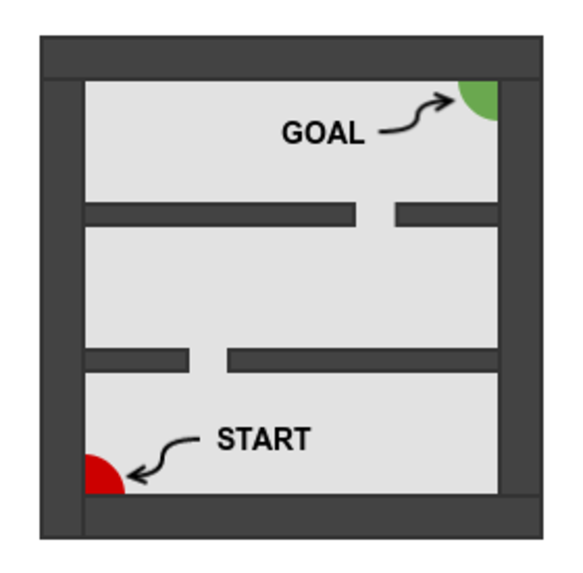
\includegraphics[trim=1.0cm 0.9cm 1.0cm 0.9cm,clip=true,height=2.5cm]{images/rooms.pdf} \hfill
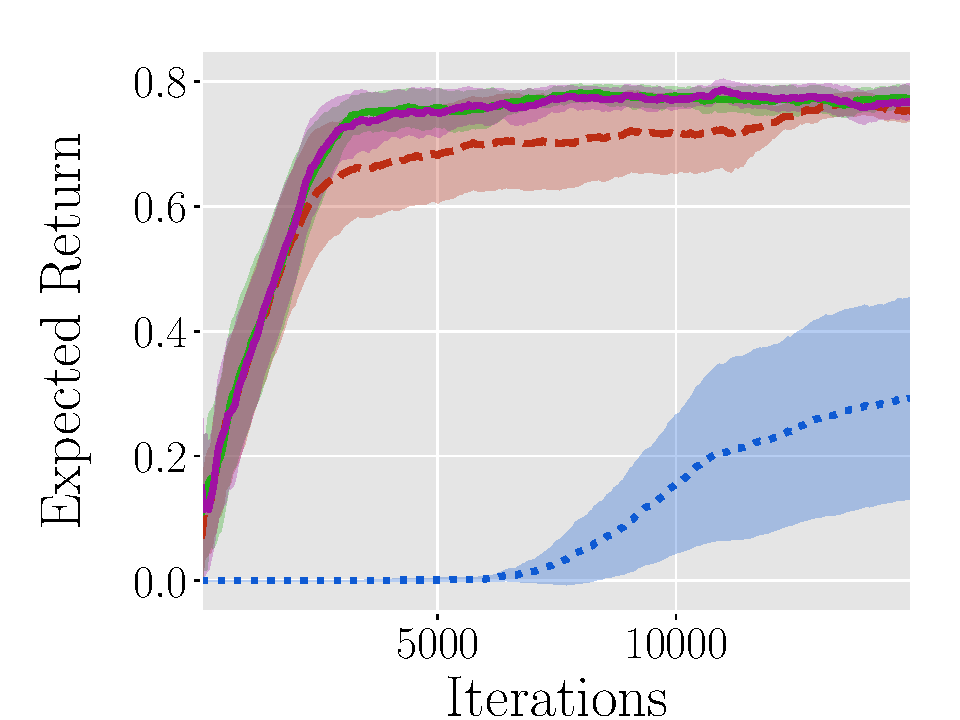
\includegraphics[trim=0.5cm 0cm 1.8cm 1.3cm,clip=true,height=2.5cm]{images/three-room/lrev.pdf}
\caption{Bla bla bla}
    \label{fig:puddleworld}
\end{minipage}\hfill
\begin{minipage}[t]{0.49\linewidth}
\centering
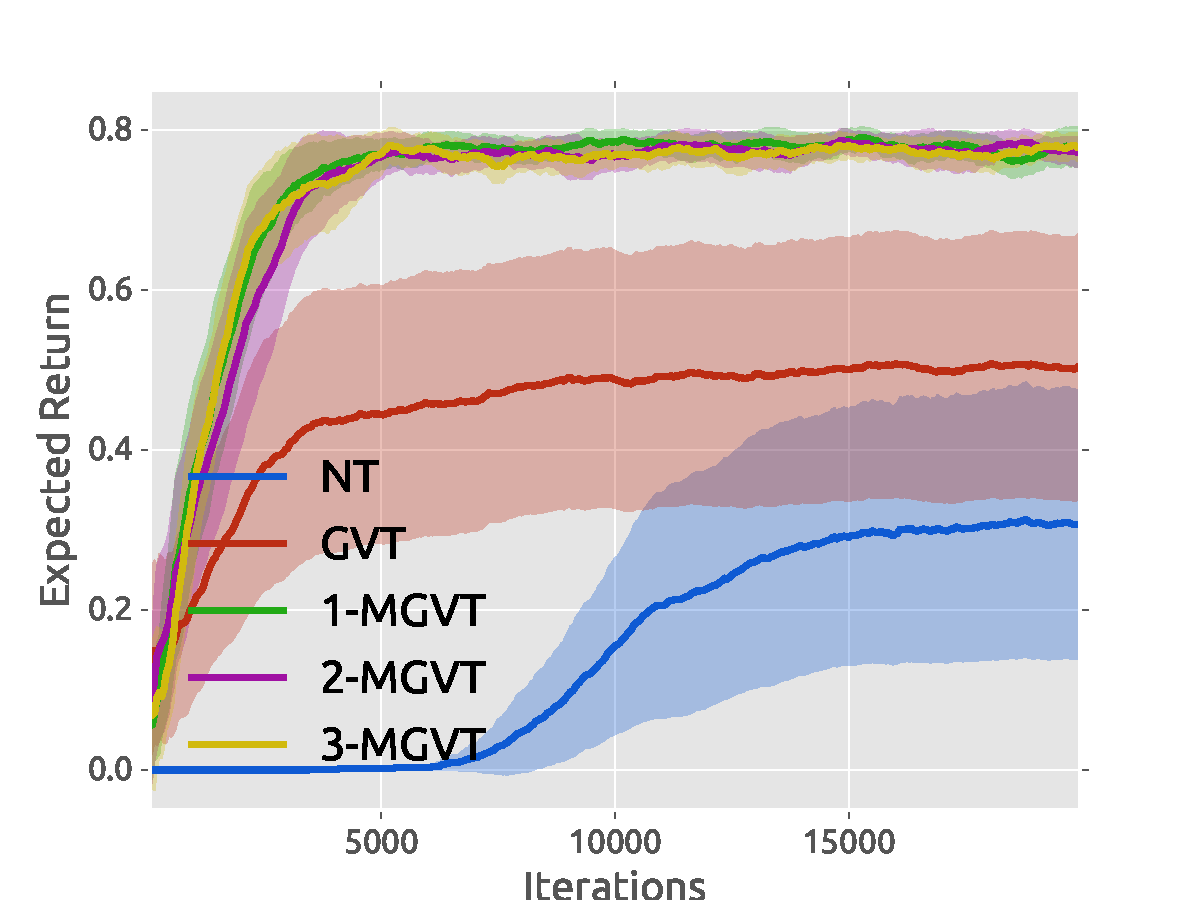
\includegraphics[trim=0.5cm 0cm 1.6cm 1.3cm,clip=true,height=2.5cm]{images/three-room-gen/lrev.pdf} \hfill
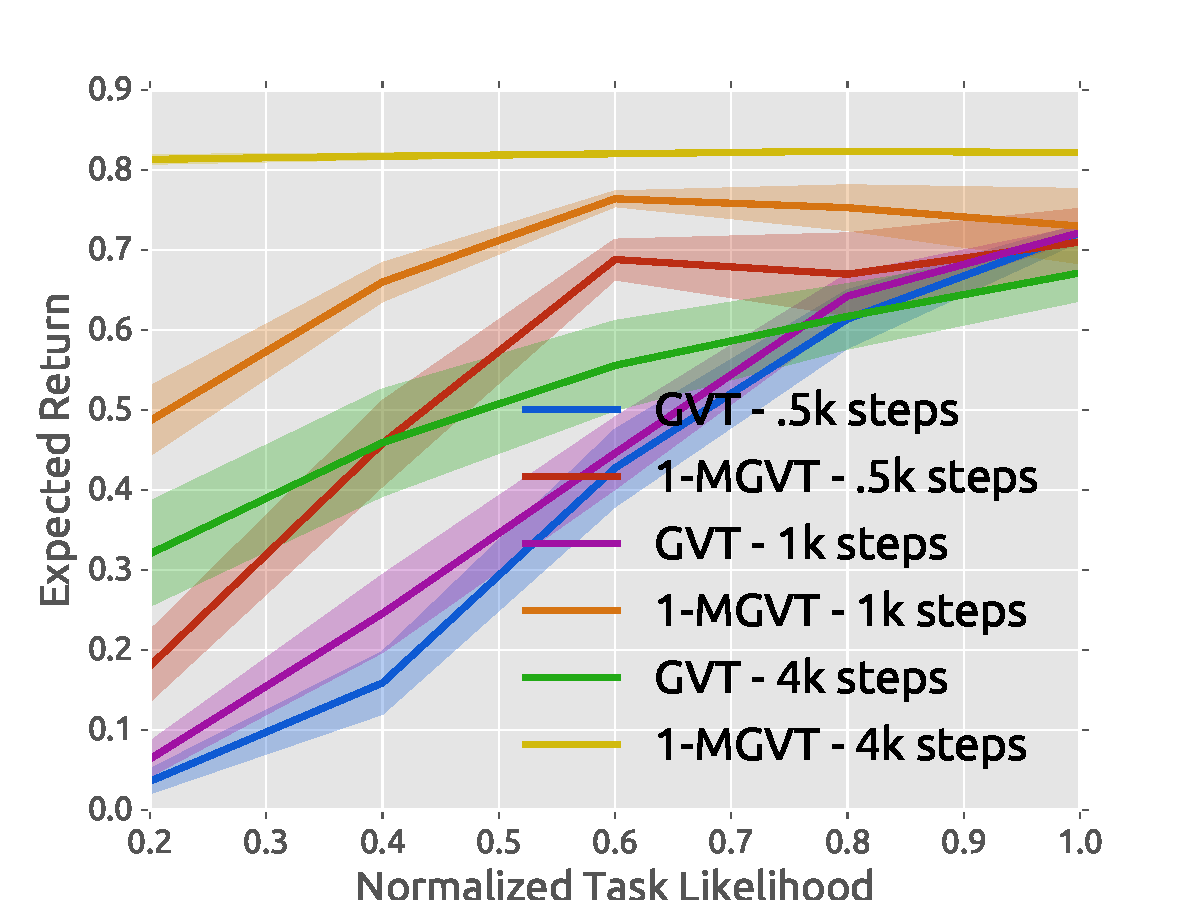
\includegraphics[trim=0.5cm 0cm 1.6cm 1.3cm,clip=true,height=2.5cm]{images/likelihood/lrew.pdf}
\caption{Bla bla bla}
    \label{fig:acrobot}
\end{minipage}
\end{figure*}

We consider an agent navigating in the rooms environment depicted in Fig. \ref{}. The agent starts in the bottom-left corner and must move from one room to another to reach the goal position in the top-right corner. The rooms are connected by small doors whose positions are unknown to the agent. In particular, we consider two versions of the environment, with two rooms (Fig. \ref{} top) and three rooms (Fig. \ref{} bottom), respectively. The state-space is modeled as a $10 \times 10$ continuous grid, while the action-space is the set of $4$ movement directions (up, right, down, left). After each action, the agent moves by $1$ in the chosen direction and the final position is corrupted by Gaussian noise with $0.2$ standard deviation. In case the agent hits a wall, its position remains unchanged. The reward is $1$ when reaching the goal (after which the process terminates) and $0$ otherwise, while the discount factor is $\gamma = 0.99$. We consider a distribution over tasks in which doors have a fixed width of $1$, while their positions are sampled uniformly in $[0.5,9.5]$. Since the agent does not know where the doors are located in advance and receives only very sparse feedback, it must efficiently explore the environment to figure out (i) their positions, and (ii) how to reach the goal. While this might be a complicated problem for plain RL, our transfer algorithm should be able to quickly figure out the door positions. In fact, notice that, although different, the optimal $Q$-functions for all tasks share some similarities. For example, once the agent has passed the last door before the goal, the $Q$-values are exactly the same in all tasks. This does not hold for positions nearby the start state. However, it is clear that there should be a preference over actions up and right, rather than down and left (which are worse in all tasks). Thus, we expect our algorithm to efficiently explore any target task.

\subsection{Classic Control} \label{sec:cc}

\subsection{Maze Navigation} \label{sec:mn}

\section{Conclusion}

{\small 
\bibliography{biblio.bib}
\bibliographystyle{plain}
}

\newpage
\appendix

\section{Proofs}

\thmmv*
\begin{proof}
We begin by noticing that:
\begin{align*}
\norm{V-\wt{V}}_{\nu,p}^p =\ & \norm{TV - \wt{T}\wt{V}}_{\nu,p}^p \\ =\ &
\norm{TV - \wt{T}V + \wt{T}V - \wt{T}\wt{V}}_{\nu,p}^p \\ \leq\ &
\norm{TV - \wt{T}V}_{\nu,p}^p + \norm{\wt{T}V - \wt{T}\wt{V}}_{\nu,p}^p \\ \leq\ &
\norm{TV - \wt{T}V}_{\nu,p}^p + \gamma\norm{V - \wt{V}}_{\nu,p}^p
\end{align*}
where the first inequality follows from Minkowsky's inequality and the second one from the contraction property of the mellow Bellman operator. This implies that:
\begin{align} \label{eq:mm1}
\norm{V-\wt{V}}_{\nu,p}^p \leq \frac{1}{1-\gamma}\norm{TV - \wt{T}V}_{\nu,p}^p
\end{align}
Let us bound the norm on the right-hand side separately. In order to do that, we will bound the function $\abs{TV(s) - \wt{T}V(s)}$ point-wisely for any state $s$. By applying the definition of the optimal and mellow Bellman operators, we obtain:
\begin{align*}
\abs{TV(s) - \wt{T}V(s)} =\ & \abs{\max_{a}\lbrace R(s,a) + \gamma\mathbb{E}\left[V(s')\right] \rbrace - \mm_{a}\lbrace R(s,a) + \gamma\mathbb{E}\left[V(s')\right] \rbrace}\\ =\ & \abs{\max_a Q(s,a) - \mm_a Q(s,a)}
\end{align*}
Recall that applying the mellow-max is equivalent to computing an expectation under a Boltzmann distribution with inverse temperature $\beta$ induced by $\kappa$ \cite{}\todo{Cite MM}. Thus, we can write:
\begin{align} \label{eq:mm2}
\abs{\max_a Q(s,a) - \mm_a Q(s,a)} =\ & \abs{\sum_a \pi^*(a|s)Q(s,a) - \sum_a \pi_{\beta}(a|s)Q(s,a)}\notag\\ =\ & \abs{\sum_a Q(s,a) \left( \pi^*(a|s) - \pi_{\beta}(a|s)  \right)}\notag\\ \leq\ & \sum_a \abs{Q(s,a)} \abs{\pi^*(a|s) - \pi_{\beta}(a|s)}\notag\\ \leq\ & \frac{R_{max}}{1-\gamma}\sum_a\abs{\pi^*(a|s) - \pi_{\beta}(a|s)}
\end{align}
where $\pi^*$ is the optimal (deterministic) policy w.r.t. $Q$ and $\pi_{\beta}$ is the Boltzmann distribution induced by $Q$ with inverse temperature $\beta$:
\begin{align*}
\pi_{\beta}(a|s) = \frac{e^{\beta Q(s,a)}}{\sum_{a'}e^{\beta Q(s,a')}}
\end{align*}
Denote by $a_1(s)$ the optimal action for state $s$ under $Q$. We can then write:
\begin{align} \label{eq:mm3}
\sum_a\abs{\pi^*(a|s) - \pi_{\beta}(a|s)} =\ & \abs{\pi^*(a_1(s)|s) - \pi_{\beta}(a_1(s)|s)} + \sum_{a \neq a_1(s)}\abs{\pi^*(a|s) - \pi_{\beta}(a|s)}\notag\\ =\ & \abs{1 - \pi_{\beta}(a_1(s)|s)} + \sum_{a \neq a_1(s)}\abs{\pi_{\beta}(a|s)}\notag\\ =\ & 2\abs{1 - \pi_{\beta}(a_1(s)|s)}
\end{align}
Finally, let us bound this last term:
\begin{align} \label{eq:mm4}
\abs{1 - \pi_{\beta}(a_1(s)|s)} =\ & \abs{1 - \frac{e^{\beta Q(s,a_1(s))}}{\sum_{a'}e^{\beta Q(s,a')}}}\notag\\ =\ & \abs{1 - \frac{e^{\beta \left( Q(s,a_1(s)) - Q(s,a_2(s)) \right)}}{\sum_{a'}e^{\beta \left( Q(s,a') - Q(s,a_2(s))\right)}}}\notag\\ =\ & \abs{1 - \frac{e^{\beta g(s)}}{\sum_{a'}e^{\beta \left( Q(s,a') - Q(s,a_2(s))\right)}}}\notag\\ =\ & \abs{1 - \frac{e^{\beta g(s)}}{e^{\beta g(s)} + \sum_{a' \neq a_1(s)}e^{\beta \left( Q(s,a') - Q(s,a_2(s))\right)}}}\notag\\ \leq & \abs{1 - \frac{e^{\beta g(s)}}{e^{\beta g(s)} + \abs{\mathcal{A}}}}\notag\\ = & \abs{1 - \frac{1}{1 + \abs{\mathcal{A}}e^{-\beta g(s)}}}
\end{align}
Combining Eq. \eqref{eq:mm2}, \eqref{eq:mm3}, and \eqref{eq:mm4}, we obtain:
\begin{align*}
\abs{\max_a Q(s,a) - \mm_a Q(s,a)} \leq\ \frac{2R_{max}}{1-\gamma}\abs{1 - \frac{1}{1 + \abs{\mathcal{A}}e^{-\beta g(s)}}}
\end{align*}
Taking the norm and plugging this into Eq. \eqref{eq:mm1} concludes the proof.
\end{proof}

\thmm*
\begin{proof}
We begin by noticing that:
\begin{align*}
\norm{Q^*-\wt{Q}}_{\nu,p}^p =\ & \norm{TQ^* - \wt{T}\wt{Q}}_{\nu,p}^p \\ =\ &
\norm{TQ^* - \wt{T}Q^* + \wt{T}Q^* - \wt{T}\wt{Q}}_{\nu,p}^p \\ \leq\ &
\norm{TQ^* - \wt{T}Q^*}_{\nu,p}^p + \norm{\wt{T}Q^* - \wt{T}\wt{Q}}_{\nu,p}^p \\ \leq\ &
\norm{TQ^* - \wt{T}Q^*}_{\nu,p}^p + \gamma\norm{Q^* - \wt{Q}}_{\nu,p}^p
\end{align*}
where the first inequality follows from Minkowsky's inequality and the second one from the contraction property of the mellow Bellman operator. This implies that:
\begin{align} \label{eq:mm1}
\norm{Q^*-\wt{Q}}_{\nu,p}^p \leq \frac{1}{1-\gamma}\norm{TQ^* - \wt{T}Q^*}_{\nu,p}^p
\end{align}
Let us bound the norm on the right-hand side separately. In order to do that, we will bound the function $\abs{TQ^*(s,a) - \wt{T}Q^*(s,a)}$ point-wisely for any state $s,a$. By applying the definition of the optimal and mellow Bellman operators, we obtain:
\begin{align} \label{eq:mm5}
\abs{TQ^*(s,a) - \wt{T}Q^*(s,a)} =\ & \abs{R(s,a) + \gamma\mathbb{E}\left[\max_{a'}Q^*(s',a')\right] - R(s,a) - \gamma\mathbb{E}\left[\mm_{a'}Q^*(s',a')\right]}\notag \\ =\ & \gamma\abs{\mathbb{E}\left[\max_{a'}Q^*(s',a')\right] - \mathbb{E}\left[\mm_{a'}Q^*(s',a')\right]}\notag \\ \leq\ & \gamma\mathbb{E}\left[\abs{\max_{a'}Q^*(s',a') - \mm_{a'}Q^*(s',a')}\right]
\end{align}
Thus, bounding this quantity reduces to bounding $\abs{\max_{a}Q^*(s,a) - \mm_{a}Q^*(s,a)}$ point-wisely for any $s$. Recall that applying the mellow-max is equivalent to computing an expectation under a Boltzmann distribution with inverse temperature $\beta_{\kappa}$ induced by $\kappa$ \cite{}\todo{Cite MM}. Thus, we can write:
\begin{align} \label{eq:mm2}
\abs{\max_a Q^*(s,a) - \mm_a Q^*(s,a)} =\ & \abs{\sum_a \pi^*(a|s)Q^*(s,a) - \sum_a \pi_{\beta_{\kappa}}(a|s)Q^*(s,a)}\notag\\ =\ & \abs{\sum_a Q^*(s,a) \left( \pi^*(a|s) - \pi_{\beta_{\kappa}}(a|s)  \right)}\notag\\ \leq\ & \sum_a \abs{Q^*(s,a)} \abs{\pi^*(a|s) - \pi_{\beta_{\kappa}}(a|s)}\notag\\ \leq\ & \frac{R_{max}}{1-\gamma}\sum_a\abs{\pi^*(a|s) - \pi_{\beta_{\kappa}}(a|s)}
\end{align}
where $\pi^*$ is the optimal (deterministic) policy w.r.t. $Q^*$ and $\pi_{\beta_{\kappa}}$ is the Boltzmann distribution induced by $Q^*$ with inverse temperature $\beta_{\kappa}$:
\begin{align*}
\pi_{\beta}(a|s) = \frac{e^{\beta_{\kappa} Q^*(s,a)}}{\sum_{a'}e^{\beta_{\kappa} Q^*(s,a')}}
\end{align*}
Denote by $a_1(s)$ the optimal action for state $s$ under $Q^*$. We can then write:
\begin{align} \label{eq:mm3}
\sum_a\abs{\pi^*(a|s) - \pi_{\beta_{\kappa}}(a|s)} =\ & \abs{\pi^*(a_1(s)|s) - \pi_{\beta_{\kappa}}(a_1(s)|s)} + \sum_{a \neq a_1(s)}\abs{\pi^*(a|s) - \pi_{\beta_{\kappa}}(a|s)}\notag\\ =\ & \abs{1 - \pi_{\beta_{\kappa}}(a_1(s)|s)} + \sum_{a \neq a_1(s)}\abs{\pi_{\beta_{\kappa}}(a|s)}\notag\\ =\ & 2\abs{1 - \pi_{\beta_{\kappa}}(a_1(s)|s)}
\end{align}
Finally, let us bound this last term:
\begin{align} \label{eq:mm4}
\abs{1 - \pi_{\beta_{\kappa}}(a_1(s)|s)} =\ & \abs{1 - \frac{e^{\beta_{\kappa} Q^*(s,a_1(s))}}{\sum_{a'}e^{\beta_{\kappa} Q^*(s,a')}}}\notag\\ =\ & \abs{1 - \frac{e^{\beta_{\kappa} \left( Q^*(s,a_1(s)) - Q^*(s,a_2(s)) \right)}}{\sum_{a'}e^{\beta_{\kappa} \left( Q^*(s,a') - Q^*(s,a_2(s))\right)}}}\notag\\ =\ & \abs{1 - \frac{e^{\beta_{\kappa} g(s)}}{\sum_{a'}e^{\beta_{\kappa} \left( Q^*(s,a') - Q^*(s,a_2(s))\right)}}}\notag\\ =\ & \abs{1 - \frac{e^{\beta_{\kappa} g(s)}}{e^{\beta_{\kappa} g(s)} + \sum_{a' \neq a_1(s)}e^{\beta_{\kappa} \left( Q^*(s,a') - Q^*(s,a_2(s))\right)}}}\notag\\ \leq & \abs{1 - \frac{e^{\beta_{\kappa} g(s)}}{e^{\beta_{\kappa} g(s)} + \abs{\mathcal{A}}}}\notag\\ = & \abs{\frac{1}{1 + \frac{1}{\abs{\mathcal{A}}}e^{\beta_{\kappa} g(s)}}}
\end{align}
Combining Eq. \eqref{eq:mm2}, \eqref{eq:mm3}, and \eqref{eq:mm4}, we obtain:
\begin{align*}
\abs{\max_a Q(s,a) - \mm_a Q(s,a)} \leq\ \frac{2 R_{max}}{1-\gamma}\abs{\frac{1}{1 + \frac{1}{\abs{\mathcal{A}}}e^{\beta_{\kappa} g(s)}}}
\end{align*}
Finally, using Eq. \eqref{eq:mm5} we get:
\begin{align*}
\abs{TQ^*(s,a) - \wt{T}Q^*(s,a)} \leq \frac{2\gamma R_{max}}{1-\gamma}\abs{\frac{1}{1 + \frac{1}{\abs{\mathcal{A}}}e^{\beta_{\kappa} g(s)}}}
\end{align*}
Taking the norm and plugging this into Eq. \eqref{eq:mm1} concludes the proof.
\end{proof}

\begin{lemma}
Let $p$ and $\nu$ denote probability measures over $Q$-functions and state-action pairs, respectively. Assume $Q^*$ is the unique fixed-point of the optimal Bellman operator $T$. Then, for any $\delta > 0$, with probability at least $1 - \delta$ over the choice of a $Q$-function $Q$, the following holds:
\begin{equation}
\norm{Q - Q^*}_{\nu}^2 \leq \frac{\mathbb{E}_p\left[ \norm{B(Q)}_{\nu}^2 \right]}{(1-\gamma)\delta}
\end{equation}
\end{lemma}
\begin{proof}
First notice that:
\begin{align*}
\norm{Q - Q^*} =\ & \norm{Q + TQ - TQ - TQ^*}\\ \leq\ & \norm{Q - TQ} + \norm{TQ - TQ^*}\\ \leq\ & \norm{Q - TQ} + \gamma\norm{Q - Q^*}\\ =\ & \norm{B(Q)} + \gamma\norm{Q - Q^*}
\end{align*}
which implies that:
\begin{align*}
\norm{Q - Q^*} \leq\ \frac{1}{1-\gamma}\norm{B(Q)}
\end{align*}
Then we can write:
\begin{align*}
P\left( \norm{Q - Q^*} > \epsilon \right) \leq P\left(\norm{B(Q)} > \epsilon (1-\gamma)\right) \leq \frac{\mathbb{E}_p\left[ \norm{B(Q)}_{\nu}^2 \right]}{(1-\gamma)\epsilon}
\end{align*}
Settings the right-hand side equal to $\delta$ and solving for $\epsilon$ concludes the proof.
\end{proof}

\begin{corollary}
Let $p$ and $\nu$ denote probability measures over $Q$-functions and state-action pairs, respectively. Assume $\wt{Q}$ is the unique fixed-point of the mellow Bellman operator $\wt{T}$. Then, for any $\delta > 0$, with probability at least $1 - \delta$ over the choice of a $Q$-function $Q$, the following holds:
\begin{equation}
\norm{Q - \wt{Q}}_{\nu}^2 \leq \frac{\mathbb{E}_p\left[ \norm{\wt{B}(Q)}_{\nu}^2 \right]}{(1-\gamma)\delta}
\end{equation}
\end{corollary}

\begin{lemma}\label{lemma:l2}
Assume $Q$-functions belong to a parametric space of functions bounded by $\frac{R_{max}}{1-\gamma}$. Let $p$ and $q$ be arbitrary distributions over the parameter space $\mathcal{W}$, and $\nu$ be a probability measure over $\mathcal{S}\times\mathcal{A}$. Consider a dataset $D$ of $N$ samples and define $v(\bm{w}) \triangleq \mathbb{E}_{\nu}\left[Var_{\mathcal{P}}\left[b(\bm{w})\right]\right]$. Then, for any $\delta > 0$, with probability at least $1-\delta$, the following two inequalities hold simultaneously:
\begin{equation}\label{eq:lemma2-1}
\mathbb{E}_q\left[ \norm{B(\bm{w})}_{\nu}^2 \right ] \leq \mathbb{E}_q\left[ \norm{B(\bm{w})}_D^2 \right] - \mathbb{E}_q\left[ v(\bm{w}) \right] + \frac{\lambda}{N} KL(q||p) + 4\frac{R_{max}^2}{(1-\gamma)^2}\sqrt{\frac{\log\frac{2}{\delta}}{2N}}
\end{equation}
\begin{equation}\label{eq:lemma2-2}
\mathbb{E}_q\left[ \norm{B(\bm{w})}_D^2 \right] \leq \mathbb{E}_q\left[ \norm{B(\bm{w})}_{\nu}^2 \right ] + \mathbb{E}_q\left[ v(\bm{w}) \right] + \frac{\lambda}{N} KL(q||p) + 4\frac{R_{max}^2}{(1-\gamma)^2}\sqrt{\frac{\log\frac{2}{\delta}}{2N}}
\end{equation}
\end{lemma}
\begin{proof}
From Hoeffding's inequality we have:
\begin{align*}
P\left( \abs{\mathbb{E}_{\nu,\mathcal{P}}\left[\norm{B(\bm{w})}_D^2\right] - \norm{B(\bm{w})}_D^2} > \epsilon \right) \leq 2exp\left( -\frac{2N\epsilon^2}{\left(2\frac{R_{max}}{1-\gamma}\right)^4} \right)
\end{align*}
which implies that, for any $\delta>0$, with probability at least $1-\delta$:
\begin{align*}
\abs{\mathbb{E}_{\nu,\mathcal{P}}\left[\norm{B(\bm{w})}_D^2\right] - \norm{B(\bm{w})}_D^2} \leq 4\frac{R_{max}^2}{(1-\gamma)^2}\sqrt{\frac{\log\frac{2}{\delta}}{2N}}
\end{align*}
Under independence assumptions, the expected TD error can be re-written as:
\begin{align*}
\mathbb{E}_{\nu,\mathcal{P}}\left[\norm{B(\bm{w})}_D^2\right] =\ & \mathbb{E}_{\nu,\mathcal{P}}\left[\frac{1}{N}\sum_{i=1}^N (r_i + \gamma \mm_{a'} Q_{\bm{w}}(s_i',a') - Q_{\bm{w}}(s_i,a_i))^2\right]\\ =\ & \mathbb{E}_{\nu,\mathcal{P}}\left[(R(s,a) + \gamma \mm_{a'} Q_{\bm{w}}(s',a') - Q_{\bm{w}}(s,a))^2\right]\\ =\ & \mathbb{E}_{\nu}\left[\mathbb{E}_{\mathcal{P}}\left[b(\bm{w})^2\right]\right]\\ =\ & \mathbb{E}_{\nu}\left[Var_{\mathcal{P}}\left[b(\bm{w})\right] + \mathbb{E}_{\mathcal{P}}\left[b(\bm{w})\right]^2\right]\\ =\ & v(\bm{w}) + \norm{B(\bm{w})}_{\nu}^2
\end{align*}
where $v(\bm{w}) \triangleq \mathbb{E}_{\nu}\left[Var_{\mathcal{P}}\left[b(\bm{w})\right]\right]$. Thus:
\begin{align}\label{eq:hoeff}
\abs{\norm{B(\bm{w})}_{\nu}^2 + v(\bm{w}) - \norm{B(\bm{w})}_D^2} \leq 4\frac{R_{max}^2}{(1-\gamma)^2}\sqrt{\frac{\log\frac{2}{\delta}}{2N}}
\end{align}
From the change of measure inequality \cite{}\todo{Find a reference for this}, we have that, for any measurable function $f(\bm{w})$ and any two probability measures $p$ and $q$:
\begin{align*}
\log\mathbb{E}_p\left[e^{f(\bm{w})}\right] \geq \mathbb{E}_q\left[ f(\bm{w}) \right] - KL(q||p)
\end{align*}
Thus, multiplying both sides of \eqref{eq:hoeff} by $\lambda^{-1}N$ and applying the change of measure inequality with $f(\bm{w}) = \lambda^{-1}N\abs{\norm{B(\bm{w})}_{\nu}^2 + v(\bm{w}) - \norm{B(\bm{w})}_D^2}$, we obtain:
\begin{align*}
\mathbb{E}_q\left[ f(\bm{w}) \right] - KL(q||p) \leq \log\mathbb{E}_p\left[e^{f(\bm{w})}\right] \leq 4\frac{R_{max}^2 \lambda^{-1}N}{(1-\gamma)^2}\sqrt{\frac{\log\frac{2}{\delta}}{2N}}
\end{align*}
where the second inequality holds since the right-hand side of \eqref{eq:hoeff} does not depend on $\bm{w}$. Finally, we can explicitly write:
\begin{align*}
\mathbb{E}_q\left[ \abs{\norm{B(\bm{w})}_{\nu}^2 + v(\bm{w}) - \norm{B(\bm{w})}_D^2} \right] \leq \frac{\lambda}{N} KL(q||p) + 4\frac{R_{max}^2}{(1-\gamma)^2}\sqrt{\frac{\log\frac{2}{\delta}}{2N}}
\end{align*}
from which the lemma follows straightforwardly.
\end{proof}

\begin{lemma}
Let $p$ be a prior distribution over the parameter space $\mathcal{W}$, and $\nu$ be a probability measure over $\mathcal{S}\times\mathcal{A}$. Assume $\wh{\xi}$ is the minimizer of $ELBO(\xi) = \mathbb{E}_{q_{\xi}}\left[ \norm{B(\bm{w})}_D^2 \right] + \frac{\lambda}{N} KL({q_{\xi}}||p)$ for a dataset $D$ of $N$ samples. Define $v(\bm{w}) \triangleq \mathbb{E}_{\nu}\left[Var_{\mathcal{P}}\left[b(\bm{w})\right]\right]$. Then, for any $\delta > 0$, with probability at least $1-\delta$:
\begin{align*}
\mathbb{E}_{q_{\wh{\xi}}}\left[ \norm{B(\bm{w})}_{\nu}^2 \right ] \leq \inf_{\xi \in \Xi}\left\{ \mathbb{E}_{q_{\xi}}\left[ \norm{B(\bm{w})}_{\nu}^2 \right ] + \mathbb{E}_{q_{\xi}}\left[ v(\bm{w}) \right] + 2\frac{\lambda}{N} KL({q_{\xi}}||p) \right\} + 2\frac{R_{max}^2}{(1-\gamma)^2}\sqrt{\frac{\log\frac{2}{\delta}}{N}}
\end{align*}
\end{lemma}
\begin{proof}
Let us use Lemma \ref{lemma:l2} for the specific choice $q=q_{\wh{\xi}}$. From Eq. \eqref{eq:lemma2-1}, we have:
\begin{align*}
\mathbb{E}_{q_{\wh{\xi}}}\left[ \norm{B(\bm{w})}_{\nu}^2 \right ] \leq\ & \mathbb{E}_{q_{\wh{\xi}}}\left[ \norm{B(\bm{w})}_D^2 \right] - \mathbb{E}_{q_{\wh{\xi}}}\left[ v(\bm{w}) \right] + \frac{\lambda}{N} KL({q_{\wh{\xi}}}||p) + 4\frac{R_{max}^2}{(1-\gamma)^2}\sqrt{\frac{\log\frac{2}{\delta}}{2N}}\\ \leq\ & \mathbb{E}_{q_{\wh{\xi}}}\left[ \norm{B(\bm{w})}_D^2 \right] + \frac{\lambda}{N} KL({q_{\wh{\xi}}}||p) + 4\frac{R_{max}^2}{(1-\gamma)^2}\sqrt{\frac{\log\frac{2}{\delta}}{2N}}\\ =\ & \inf_{\xi \in \Xi}\left\{ \mathbb{E}_{q_{\xi}}\left[ \norm{B(\bm{w})}_D^2 \right] + \frac{\lambda}{N} KL({q_{\xi}}||p) \right\} + 4\frac{R_{max}^2}{(1-\gamma)^2}\sqrt{\frac{\log\frac{2}{\delta}}{2N}}
\end{align*}
where the second inequality holds since $v(\bm{w}) > 0$, while the equality holds from the definition of $\wh{\xi}$. We can now use Eq. \eqref{eq:lemma2-2} to bound $\mathbb{E}_{q_{\xi}}\left[ \norm{B(\bm{w})}_D^2 \right]$, thus obtaining:
\begin{align*}
\mathbb{E}_{q_{\wh{\xi}}}\left[ \norm{B(\bm{w})}_{\nu}^2 \right ] \leq \inf_{\xi \in \Xi}\left\{ \mathbb{E}_{q_{\xi}}\left[ \norm{B(\bm{w})}_{\nu}^2 \right ] + \mathbb{E}_{q_{\xi}}\left[ v(\bm{w}) \right] + 2\frac{\lambda}{N} KL({q_{\xi}}||p) \right\} + 2\frac{R_{max}^2}{(1-\gamma)^2}\sqrt{\frac{\log\frac{2}{\delta}}{N}}
\end{align*}
This concludes the proof.
\end{proof}

\section{Additional Details on the Experiments}

\subsection{The Rooms Problem}

\subsection{Classic Control}

\subsection{Maze Navigation}

Transfer approaches to mention:
\begin{itemize}
\item Taylor 2009: survey
\item Konidaris and Barto transfer shaped reward functions PROs: this allows the agent to have a more goal-directed behavior, thus limiting unnecessary random exploration CONs: applicable only to simple problems, does not scale
\item Wilson 2007 propose a hierarchical Bayesian model for the distribution over tasks PROs it explicitly models the uncertainty over which tasks are being solved, thus quickly adapting to new ones and allowing informed exploration decisions to be taken
\item Lazaric 2008 transfer samples PROs select good samples, can scale to continuous domains CONs eps greedy is used
\item Taylor 2008 transfer samples for model-based RL PROs good exploration via model-based RL CONs does not scale, can negatively transfer when tasks are very different
\item Lazaric 2010 propose a hierarchical bayesian model for the distribution over value functions PROs quickly adapts to new tasks, non-parameteric (GP) models CONs scaling, strong assumptions (GPTD)
\item Fernandez and veloso 2006 propose an exploration strategy based on probabilistic policy reuse PROs good exploration (?) CONs Do not try to figure out which policies are good or bad
\item Brunskill propose a method to transfer in model based RL (E3) - PROs theory, exploration CONs scaling
\item Barreto use successor features PROs simple, theory CONs eps-greedy exploration
\end{itemize}

Exploration approaches to mention:
\begin{itemize}
\item Osband 2014 propose a method to efficiently explore via randomized value functions
\item Osband 2016 adapt such algorithm to DQNs
\item Houthooft 2016 use variational inference to approximate the posterior distribution over parameters of the dynamics, and use that to drive exploration
\item Azizzadenesheli 2018 extend Osband 2016 to use Bayesian DQN instead. Still makes Gaussian assumptions though
\end{itemize}

\end{document}